\documentclass[14pt]{extbook}
\usepackage{multicol, enumerate, enumitem, hyperref, color, soul, setspace, parskip, fancyhdr} %General Packages
\usepackage{amssymb, amsthm, amsmath, bbm, latexsym, units, mathtools} %Math Packages
\everymath{\displaystyle} %All math in Display Style
% Packages with additional options
\usepackage[headsep=0.5cm,headheight=12pt, left=1 in,right= 1 in,top= 1 in,bottom= 1 in]{geometry}
\usepackage[usenames,dvipsnames]{xcolor}
\usepackage{dashrule}  % Package to use the command below to create lines between items
\newcommand{\litem}[1]{\item#1\hspace*{-1cm}\rule{\textwidth}{0.4pt}}
\pagestyle{fancy}
\lhead{Progress Quiz 5}
\chead{}
\rhead{Version A}
\lfoot{9912-2038}
\cfoot{}
\rfoot{Spring 2021}
\begin{document}

\begin{enumerate}
\litem{
Determine the vertical asymptotes and holes in the rational function below.\[ f(x) = \frac{6x^{3} +7 x^{2} -43 x -30}{8x^{2} -30 x + 25} \]\begin{enumerate}[label=\Alph*.]
\item \( \text{Vertical Asymptotes of } x = 1.25 \text{ and } x = -0.667 \text{ with a hole at } x = 2.5 \)
\item \( \text{Holes at } x = 1.25 \text{ and } x = 2.5 \text{ with no vertical asymptotes.} \)
\item \( \text{Vertical Asymptote of } x = 1.25 \text{ and hole at } x = 2.5 \)
\item \( \text{Vertical Asymptote of } x = 0.75 \text{ and hole at } x = 2.5 \)
\item \( \text{Vertical Asymptotes of } x = 1.25 \text{ and } x = 2.5 \text{ with no holes.} \)

\end{enumerate} }
\litem{
Determine the vertical asymptotes and holes in the rational function below.\[ f(x) = \frac{8x^{3} +34 x^{2} -7 x -60}{16x^{2} -32 x + 15} \]\begin{enumerate}[label=\Alph*.]
\item \( \text{Vertical Asymptotes of } x = 0.75 \text{ and } x = 1.25 \text{ with no holes.} \)
\item \( \text{Vertical Asymptote of } x = 0.75 \text{ and hole at } x = 1.25 \)
\item \( \text{Vertical Asymptote of } x = 0.5 \text{ and hole at } x = 1.25 \)
\item \( \text{Holes at } x = 0.75 \text{ and } x = 1.25 \text{ with no vertical asymptotes.} \)
\item \( \text{Vertical Asymptotes of } x = 0.75 \text{ and } x = -1.5 \text{ with a hole at } x = 1.25 \)

\end{enumerate} }
\litem{
Determine the horizontal and/or oblique asymptotes in the rational function below.\[ f(x) = \frac{6x^{3} -49 x^{2} +125 x -100}{6x^{3} -5 x^{2} -45 x + 100} \]\begin{enumerate}[label=\Alph*.]
\item \( \text{Vertical Asymptote of } y = -2.500  \)
\item \( \text{Horizontal Asymptote of } y = 1.000  \)
\item \( \text{Vertical Asymptote of } y = 4  \)
\item \( \text{None of the above} \)
\item \( \text{Horizontal Asymptote of } y = 0  \)

\end{enumerate} }
\litem{
Determine the vertical asymptotes and holes in the rational function below.\[ f(x) = \frac{8x^{3} -14 x^{2} -35 x + 50}{6x^{2} -19 x + 10} \]\begin{enumerate}[label=\Alph*.]
\item \( \text{Vertical Asymptote of } x = 1.333 \text{ and hole at } x = 2.5 \)
\item \( \text{Vertical Asymptotes of } x = 0.667 \text{ and } x = 1.25 \text{ with a hole at } x = 2.5 \)
\item \( \text{Holes at } x = 0.667 \text{ and } x = 2.5 \text{ with no vertical asymptotes.} \)
\item \( \text{Vertical Asymptotes of } x = 0.667 \text{ and } x = 2.5 \text{ with no holes.} \)
\item \( \text{Vertical Asymptote of } x = 0.667 \text{ and hole at } x = 2.5 \)

\end{enumerate} }
\litem{
Determine the vertical asymptotes and holes in the rational function below.\[ f(x) = \frac{8x^{3} -46 x^{2} +81 x -45}{8x^{2} -18 x + 9} \]\begin{enumerate}[label=\Alph*.]
\item \( \text{Holes at } x = 0.75 \text{ and } x = 1.5 \text{ with no vertical asymptotes.} \)
\item \( \text{Vertical Asymptotes of } x = 0.75 \text{ and } x = 1.5 \text{ with no holes.} \)
\item \( \text{Vertical Asymptotes of } x = 0.75 \text{ and } x = 1.25 \text{ with a hole at } x = 1.5 \)
\item \( \text{Vertical Asymptote of } x = 0.75 \text{ and hole at } x = 1.5 \)
\item \( \text{Vertical Asymptote of } x = 1.0 \text{ and hole at } x = 1.5 \)

\end{enumerate} }
\litem{
Which of the following functions \textit{could} be the graph below?
\begin{center}
    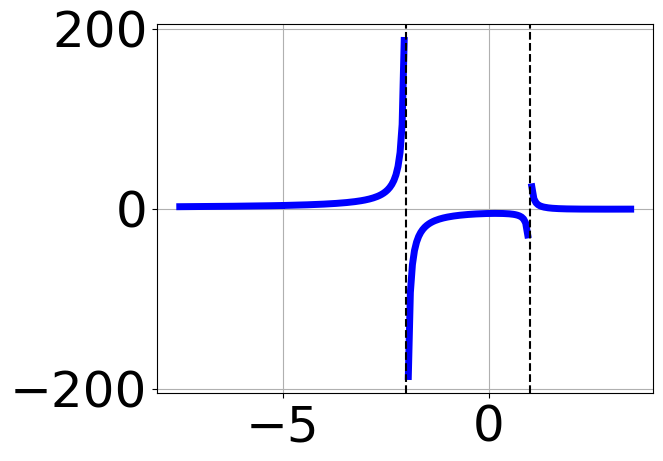
\includegraphics[width=0.5\textwidth]{../Figures/identifyGraphOfRationalFunctionCopyA.png}
\end{center}
\begin{enumerate}[label=\Alph*.]
\item \( f(x)=\frac{x^{3} -2 x^{2} -25 x + 50}{x^{3} +6 x^{2} +3 x -10} \)
\item \( f(x)=\frac{x^{3} +2 x^{2} -25 x -50}{x^{3} -6 x^{2} +3 x + 10} \)
\item \( f(x)=\frac{x^{3} -11 x^{2} +38 x -40}{x^{3} +6 x^{2} +3 x -10} \)
\item \( f(x)=\frac{x^{3} +2 x^{2} -25 x -50}{x^{3} -6 x^{2} +3 x + 10} \)
\item \( \text{None of the above are possible equations for the graph.} \)

\end{enumerate} }
\litem{
Determine the horizontal and/or oblique asymptotes in the rational function below.\[ f(x) = \frac{6x^{3} -17 x^{2} -3 x + 20}{3x^{2} -19 x + 20} \]\begin{enumerate}[label=\Alph*.]
\item \( \text{Horizontal Asymptote at } y = 5.0 \)
\item \( \text{Horizontal Asymptote of } y = 5.0 \text{ and Oblique Asymptote of } y = 2x + 7 \)
\item \( \text{Horizontal Asymptote of } y = 2.0 \text{ and Oblique Asymptote of } y = 2x + 7 \)
\item \( \text{Oblique Asymptote of } y = 2x + 7. \)
\item \( \text{Horizontal Asymptote of } y = 2.0  \)

\end{enumerate} }
\litem{
Determine the horizontal and/or oblique asymptotes in the rational function below.\[ f(x) = \frac{30x^{3} -119 x^{2} -24 x + 80}{-24x^{3} -28 x^{2} +42 x -40} \]\begin{enumerate}[label=\Alph*.]
\item \( \text{Horizontal Asymptote of } y = -1.250  \)
\item \( \text{Vertical Asymptote of } y = 0.500  \)
\item \( \text{Vertical Asymptote of } y = 4  \)
\item \( \text{None of the above} \)
\item \( \text{Horizontal Asymptote of } y = 0  \)

\end{enumerate} }
\litem{
Determine the horizontal and/or oblique asymptotes in the rational function below.\[ f(x) = \frac{8x^{3} -2 x^{2} -43 x + 30}{4x^{2} +9 x -9} \]\begin{enumerate}[label=\Alph*.]
\item \( \text{Horizontal Asymptote of } y = 2.0 \text{ and Oblique Asymptote of } y = 2x -5 \)
\item \( \text{Oblique Asymptote of } y = 2x -5. \)
\item \( \text{Horizontal Asymptote at } y = -3.0 \)
\item \( \text{Horizontal Asymptote of } y = -3.0 \text{ and Oblique Asymptote of } y = 2x -5 \)
\item \( \text{Horizontal Asymptote of } y = 2.0  \)

\end{enumerate} }
\litem{
Which of the following functions \textit{could} be the graph below?
\begin{center}
    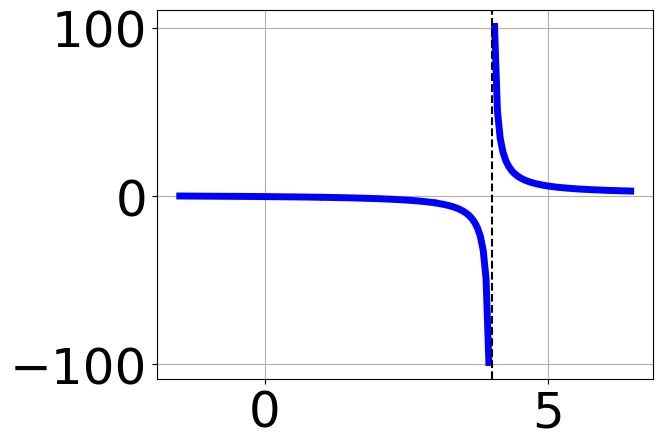
\includegraphics[width=0.5\textwidth]{../Figures/identifyGraphOfRationalFunctionA.png}
\end{center}
\begin{enumerate}[label=\Alph*.]
\item \( f(x)=\frac{x^{3} -3 x^{2} -x + 3}{x^{3} -8 x^{2} +19 x -12} \)
\item \( f(x)=\frac{x^{3} +3 x^{2} -x -3}{x^{3} +8 x^{2} +19 x + 12} \)
\item \( f(x)=\frac{x^{3} -7 x^{2} +4 x + 12}{x^{3} -8 x^{2} +19 x -12} \)
\item \( f(x)=\frac{x^{3} +3 x^{2} -x -3}{x^{3} +8 x^{2} +19 x + 12} \)
\item \( \text{None of the above are possible equations for the graph.} \)

\end{enumerate} }
\end{enumerate}

\end{document}